\documentclass[a4paper,12pt]{article}
\usepackage[margin=1in]{geometry}

\usepackage[T2A]{fontenc}			% кодировка
\usepackage[utf8]{inputenc}			% кодировка исходного текста
\usepackage[english,russian]{babel}	% локализация и переносы
\usepackage{graphicx}                % Математика
\usepackage{amsmath,amsfonts,amssymb,amsthm,mathtools} 
\usepackage{mathtext}
\usepackage[T2A]{fontenc}
\usepackage[utf8]{inputenc}

\usepackage{wasysym}

%Заговолок
\author{Бичина Марина 
группа Б04-005 1 курса ФЭФМ}
\title{}
\date{}


\begin{document} % начало документа

\begin{center}
\begin{Large}
{Корнеев Николай Б04-005, Лабораторная работа №.4.5.3 Сканирующий интерферометр}
\end{Large}
\end{center}
\paragraph{Цель работы:} 
\begin{enumerate}
\itemsep0em
\item Ознакомиться с устройством и работой газового лазера непрерывного действия
\item Ознакомиться со спектральными характеристиками лазерного излучения
\item Разобраться с устройством и принципом действия сканирующего интерферометра Фабри-Перо
\item Определить  межмодовое расстояние и приборную ширину отдельной моды излучения лазера
\item Оценить газокинетическую температуру в разряде
\item Рассчитать дисперсионную область, разрешающую способность и коэффициент отражения зеркал сканирующего интерферометра 
\end{enumerate}
\paragraph{Оборудование:}
\begin{enumerate}
\itemsep0em
\item He-Ne-лазер с блоком питания
\item сканирующий интерферометр Фабри-Перо
\item поляроид
\item пластинка $\lambda/4$
\item линза
\item фотодиод
\item электронный осциллограф
\end{enumerate}


\paragraph{Теоретическая справка:}
\begin{enumerate}
\itemsep0em
\item
Лазер, или оптический квантовый генератор, — источник квазимонохроматического и узконаправленного высококогерентного потока излучения, работающий за счёт квантово-механического эффекта индуцированного излучения.

Главными элементами лазера являются оптический резонатор и расположенная в нём активная среда, способная усиливать проходящее через неё излучения.
В He–Ne-лазерах используются резонаторы, фактически представляющие собой резонатор Фабри—Перо (информация о нем представлена ниже в описании установки). Его устройство представляет  два плоских зеркала с высокими коэффициентами отражения, размещённых параллельно друг другу на фиксированном расстоянии 

Сканирующий интерферометр, применяемый в настоящей работе, имеет зеркала с коэффициентом отражения $r\approx 98,5\%$, поэтому
с его помощью можно разрешить две узкие спектральные линии, отличающиеся по частоте на величину порядка $\sim 0,005\Delta \nu$. Таким образом, наш сканирующий интерферометр вполне подходит для исследования модового
состава лазерного излучения.
\item
\paragraph{Описание установки:}
\begin{enumerate}
\itemsep0em
\item \textbf{Резонатор Фабри-Перо}\\
Данная установка представляет из себя 2 отполированные (стеклянные или кварцевые) пластины, которые установлены $\parallel$ друг другу на некотором расстоянии. На одну из поверхностей каждых из 2-х пластин нанесено отражающее покрытие.\\
Интерференционные максимумы будут наблюдаться для волн, падающими под углами $\theta_{m}$ и удовлетворяющие условию (где L - база интерферометра)
\begin{equation}
2Lcos\theta_m = m\lambda\;\;\;\;\;\;\;m \in N
\end{equation} 
В нашем случае, мы можем считать, что $m \approx M = \frac{2L}{\lambda}$, поскольку в нашем случае зеркала расположены перпендикулярно лучу лазера.
\begin{figure}[h!]
\centering
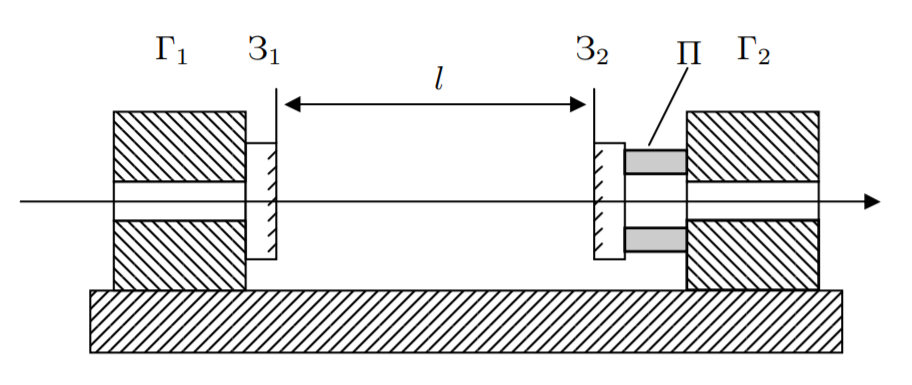
\includegraphics[scale=0.5]{../../4_term/4_5_3/setupp.png}
\caption{Сканирующий интерферометр}
\end{figure}
\item \textbf{Сканирующий интерферометр}\\
На жёстком массивном основании расположены две юстировочные
головки Г$_1$ и Г$_2$, на которых укреплены зеркала З$_1$ и З$_2$. Зеркало З$_1$ установлено непосредственно на головке Г$_1$, зеркало З$_2$ связано с головкой Г$_2$ через пьезокерамический элемент П. Юстировочные головки снабжены винтами, не показанными на рисунке, которые позволяют в
небольших пределах поворачивать зеркала относительно вертикальной
и горизонтальной осей. С помощью головок Г$_1$ и Г$_2$ зеркала выставляются на параллельность.
Пьезокерамический элемент П позволяет периодически изменять
базу интерферометра (l=10 см) на величину порядка длины световой волны, чтобы изменять пропускающую частоту. Элемент имеет форму полого цилиндра. Его внутренняя и
наружная поверхности металлизированы и образуют цилиндрический конденсатор.
Если вдоль оси интерферометра распространяется световое излучение с длиной волны $\lambda$, то при выполнении условия 
\begin{equation}
2l = m\lambda
\end{equation}
Что аналогично условию для лазера, возникает резонанс.

Собственные моды интерферометра, называемые дисперсионной областью, отличаются на величину
\begin{equation*}
\Delta \nu = \frac{c}{2L}
\end{equation*}
Они соответствуют нескольким резонансам при излучении разными длинами волн.

В единицах $\lambda$:
\begin{equation}
\Delta \lambda_{\text{си}} = \frac{\lambda^2}{2l}
\end{equation}
Разрешающая способность интерферометра Фабри-Перо задается выражением:
\begin{equation}
R=\frac{\lambda}{\delta \lambda}
\end{equation}
где $\delta \lambda$ -- минимальная разность длины волн, разрешаемая прибором вблизи длины волны $\lambda$

Разрешающая способность интерферометра Фабри-Перо зависит от длины интерферометра l и коэффициента отражения зеркал 
\begin{equation}
R = \frac{2\pi l}{\lambda(1-r)}
\end{equation}
\item \textbf{Описание установки для исследования спектрального состава излучения лазера (далее рабочая установка)}\\
\begin{figure}[h!]
\centering
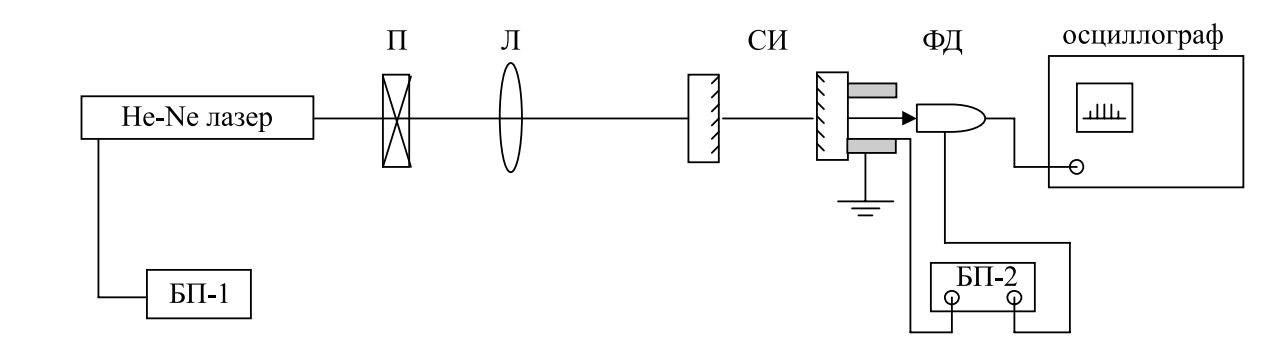
\includegraphics[scale=0.5]{../../4_term/4_5_3/setup.png}
\caption{Рабочая установка}
\end{figure}
Излучение He–Ne-лазера проходит через поляризационную развязку
и линзу(попадание на развязку предотвращает попадание в лазер излучения, отразившегося от элементов оптического тракта, линза собирает пучок, чтобы он меньше расходился), и далее поступает на вход сканирующего интерферометра.
Поляризационная развязка предотвращает попадание в лазер излучения, отразившегося от элементов оптического тракта.

Излучение, прошедшее сквозь сканирующий интерферометр, поступает на фотодиод ФД. Напряжение с фотодиода через усилитель подаётся на вертикальный вход электронного осциллографа.

Лазер питается от блока питания БП-1, фотодиод и уситилитель -- от БП-2. Напряжение на пьезоэлемент регулируется ручкой 1 и подается с БП-2
\end{enumerate}
\item \textbf{Параметры установки:}
\begin{enumerate}
\itemsep0em
\item Длина лазера $L=65$ см
\item Длина интерферометра $l = 9$ см
\item Длина волны лазера $\lambda = 632.8$ нм
\end{enumerate}
\end{enumerate}
\paragraph{Ход работы:}
\begin{enumerate}
\itemsep0em
\item Займемся калибровкой: линзу,находящуюся под лучом, временно выведем с помощью поперечных салазок. Далее совместим прямой и отражённый пучки, осторожно вращая винты 1
и 2 на первом (по ходу луча) зеркале интерферометра: два пятна на
пластинке $\lambda/4$ должны совпадать. Затем винтами 1 и 2 второго зеркала
совместим пятна на первом зеркале. Настроим поляризационную развязку.
\item Вращая ФД вверх-вних и в сторону получим на экране осциллограмму. Добьемся максимального сигнала.
\item Введем линзу, для уменьшения расходимости пучка.
\item Рассчитаем межмодовое расстояние лазера в единицах $\nu$ и $\lambda$
\[\Delta \nu =\frac{c}{2L}=\frac{c}{1.3}Hz\approx 231\;\;MHz\]
\[\nu = \frac{c}{\lambda}\approx 4.7376 \cdot 10^{14}\;\; Hz\]
\[\Delta \lambda = \lambda\frac{\Delta\nu}{\nu}=\frac{\lambda^2}{2L}=\frac{(632.8 \cdot 10^{-9})^2}{1.3}\approx 3.08 \cdot 10^{-13}\;\;\text{м}\]
\begin{figure}[h!]
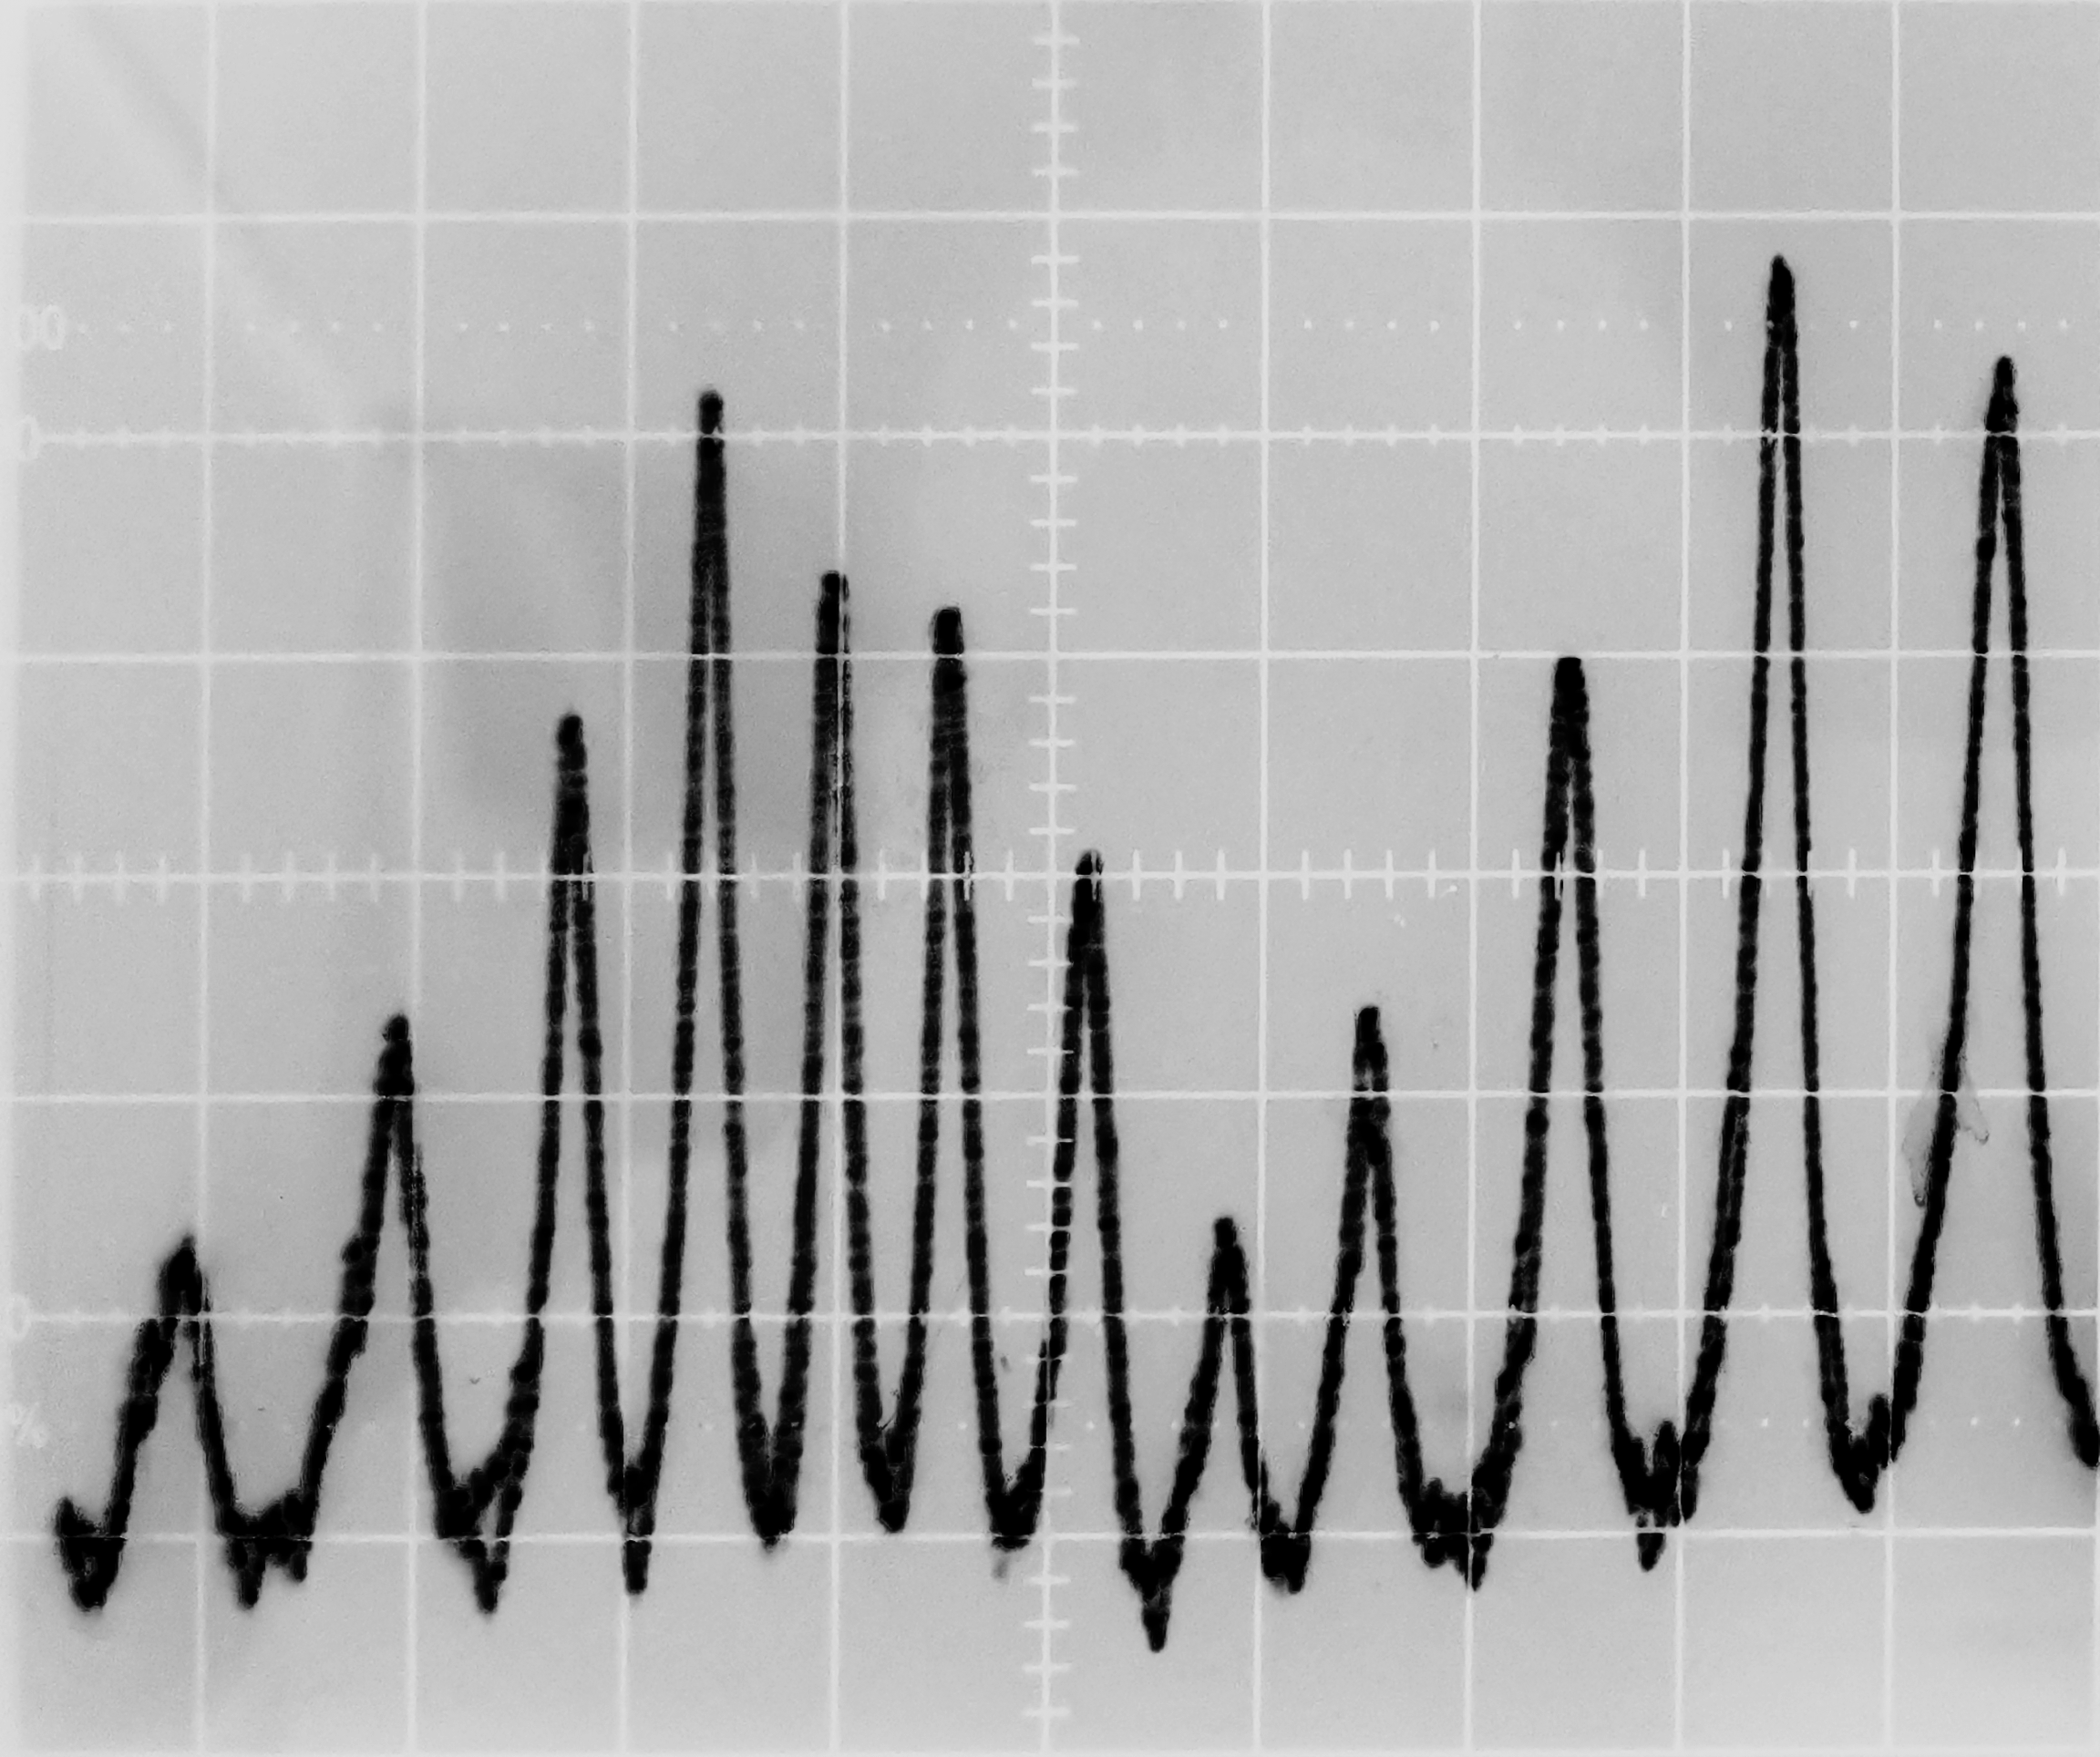
\includegraphics[scale=0.15]{wave.png} 
\centering
\end{figure}
\item Рассмотрим осциллограмму: Видим, что ширина спектральной линии неона $\Delta \nu_{Ne}$ при числе промежутков $n=6$ равна:
\[\Delta \nu_{Ne} = 6\Delta \nu=6\cdot 231 \approx 1.38\;\; GHz\]
\[\Delta \lambda_{Ne} = 6\lambda = 6\cdot 3.08 \cdot 10^{-13}\approx 18.4 \cdot 10^{-13}\;\; m\]
\item  Положим, что ширина спектральной линии обусловлена эффектом Доплера и что видимая ширина линии неона порядка полуширины доплеровского контура ($2\Delta\lambda_{D}\approx\Delta\lambda_{Ne}$). Тогда оценим среднюю скорость атомов неона $\upsilon_{x}$ газокинетическую температуру по формулам:
\[\frac{m\upsilon_{x}^2}{2}=\frac{kT}{2}\;\;\;\;\;\frac{\Delta\nu_{D}}{\nu}\approx\frac{\upsilon_{x}}{c}\]
Получим:
\[\upsilon_{x}\approx c\frac{\Delta\nu_{Ne}}{2\nu}=\frac{c\cdot 0.69\cdot 10^9}{4.737\cdot 10^{14}}\approx437\;\;m/s\]
\[T\approx\frac{3.3532\cdot 10^{-26}\cdot 190969}{13.8}\approx 464\;\;K\]
Рассчитаем дисперсионную область $\Delta\lambda_{\text{СИ}}$ по формуле 3:
\[\Delta\lambda_{\text{СИ}} = \frac{\lambda^2}{2l}=\frac{632.8^2\cdot 10^{-18}}{2\cdot 0.09}\approx 2.2\cdot 10^{12}\;\;m\]
При сравнении со значением шириной линии неона $\Delta \lambda_{Ne} \approx 1.8 \cdot 10^{-12}$ видим, что значения весьма близки
\item Сравним ширину моды на полувысоте с межмодовым расстоянием, найдем разрешающую способность R по формуле (4). 

На графике $2\delta\nu = 0.2$ дел, $\Delta \nu = 0.65$ дел, поэтому 
\[\delta\nu = \frac{0.1}{0.65}\Delta\nu\]
Тогда 
\[\delta \lambda\ = \delta\nu = 0.15\cdot 3.08\cdot 10^{-13}\approx 5 \cdot 10^{-14}m\]

\[R = \dfrac{\lambda}{\delta \lambda}=\dfrac{6.3\cdot 10^{-7}}{5\cdot 10^{-14}}= 1.26 \cdot 10^7\approx 10^7\]
\item Сделаем оценку коэффициента отражения r по формуле (5):
\[r = 1 - \frac{2\pi l}{\lambda R}=\frac{2\pi\cdot 0.09}{6.3\cdot 10^{-7}\cdot 10^7}\approx 0.9\]
\end{enumerate}
\paragraph{Выводы:}
\begin{enumerate}
\item Мы определили межмодовое расстояние $\Delta \nu = 231\;\; MHz$, $\Delta\lambda = 3.08 \cdot10^{-13}\;\;m$
\item Определили приборную ширину отдельной моды излучения лазера $\Delta \nu_{Ne} = 1.38\;\; GHz$, $\Delta \lambda_{Ne} = 18.4 \cdot 10^{-13}m$
\item Рассчитали газокинетическую температуру $T=464\;\; K$
\item Дисперсионная область:  $\Delta\lambda_{\text{СИ}} = 2.2 \cdot 10^{12} m $
\item Разрешающая способность $R = 1.26 \cdot 10^7$
\item Коэффициент отражения $r=0.9$
\end{enumerate}
\end{document}
